\part{Sexto semestre}
\chapterimage{1.pdf}
\chapter{Cálculo Integral}

\section{Diferencial de una función} % (4 horas), 3 clases
\subsection{Concepto de diferencial de una función}
\begin{definition}[Diferencial de una función]
    Sea $f: \mathbb{R} \rightarrow \mathbb{R}$ una función diferenciable en un intervalo abierto $I$ y sea $x \in I$. El diferencial de $f$ en el punto $x$, denotado por $\mathrm{d}f(x)$ o $df$, es una función lineal que aproxima el cambio en el valor de $f$ debido a un pequeño cambio en $x$. Formalmente, se define como:
\begin{equation}
    \mathrm{d}f(x) = f'(x) \, \mathrm{d}x
\end{equation}
\begin{notation}
donde:
    \begin{itemize}
        \item $f'(x)$ es la derivada de \( f \) con respecto a \( x \).
        \item $dx$ es un pequeño cambio en \( x \).
    \end{itemize}
\end{notation}
\end{definition}
\begin{example}
    Consideremos la función \( f(x) = x^2 \). Su derivada es \( f'(x) = 2x \). Entonces, la diferencial \( dy \) es:
    \begin{equation}
        dy = f'(x) \, dx = 2x \, dx
    \end{equation}
    Esto significa que para un pequeño cambio \( dx \) en \( x \), el cambio correspondiente en \( y \) es aproximadamente \( 2x \, dx \).
    
    \textbf{Aplicación}
    
    Si \( x = 3 \) y \( dx = 0.1 \):
\begin{equation*}
    dy = 2 \cdot 3 \cdot 0.1 = 0.6
\end{equation*}
    Así, cuando \( x \) cambia de 3 a 3.1, el cambio en \( y \) es aproximadamente 0.6.
\end{example}
\newpage
\subsubsection{Actividad en Matlab}
Crea una gráfica de la función $f(x) = x^2$ y su recta tangente en un punto
\begin{lstlisting}[style=Matlab-editor]
% differential_example.m

% Define the function and its derivative
f = @(x) x.^2;
df = @(x) 2*x;

% Define the point at which to evaluate the differential
x0 = 2;
y0 = f(x0);
slope = df(x0);

% Create a range of x values
x = linspace(0, 4, 100);

% Evaluate the function
y = f(x);

% Evaluate the tangent line
tangent = y0 + slope * (x - x0);

% Plot the function and the tangent line
figure;
plot(x, y, 'b-', 'LineWidth', 2);
hold on;
plot(x, tangent, 'r--', 'LineWidth=2);
plot(x0, y0, 'ko', 'MarkerFaceColor', 'k');
hold off;

% Labels and title
xlabel('x');
ylabel('y');
title('Function f(x) = x^2 and its Tangent Line at x = 2');
legend('f(x) = x^2', 'Tangent Line', 'Point of Tangency');

% Save the plot as an image
saveas(gcf, 'differential_example.png');
\end{lstlisting}
% TODO PONER PLOT
\newpage
\subsection{Interpretación geométrica en todos los posibles casos de curvas}
El diferencial se puede tomar en el sentido geométrico como la elevación de la tangente desde el punto en que se toma el diferencial.

Recuérdese que la derivada de la función en el punto es la pendiente de la recta tangente a la función en el punto, como sabemos que la tangente de un ángulo es igual al cociente entre el cateto opuesto (incremento de y) y el cateto contiguo (incremento de x) de un hipotético triángulo rectángulo, solo hay que despejar el incremento de y que equivale a nuestro diferencial.

Vista geométricamente, la elevación se produce verticalmente a partir del punto en que se toma el diferencial. El incremento $\Delta x$ que se tome representará el alejamiento horizontal que haga desde el punto en cuestión.
\begin{center}
    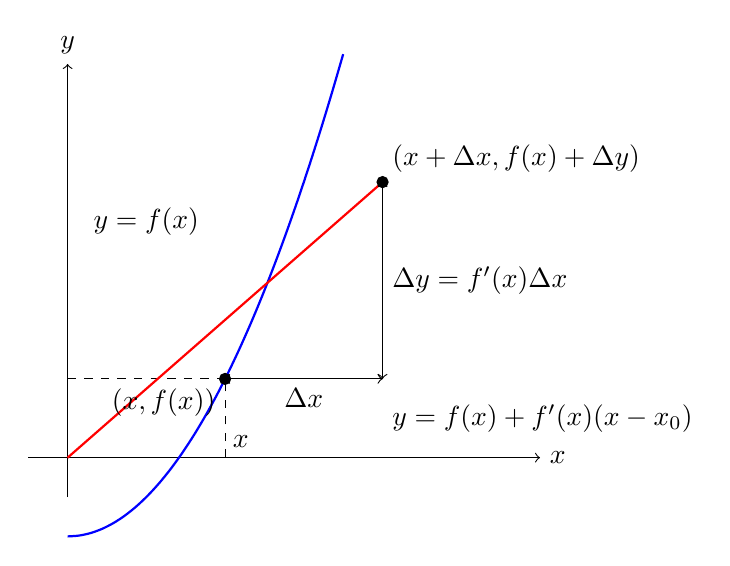
\begin{tikzpicture}
    
        % Ejes
        \draw[->] (-0.5,0) -- (6,0) node[right] {$x$};
        \draw[->] (0,-0.5) -- (0,5) node[above] {$y$};
    
        % Curva
        \draw[scale=1,domain=0:3.5,smooth,variable=\x,blue,thick] plot ({\x},{0.5*\x*\x - 1});
        
        % Punto y tangente
        \draw[dashed] (2,0) -- (2,1);
        \draw[dashed] (0,1) -- (2,1);
        \draw[red,thick] (0,0) -- (4,3.5);
        \filldraw[black] (2,1) circle (2pt) node[anchor=north east] {$(x, f(x))$};
        \filldraw[black] (4,3.5) circle (2pt) node[anchor=south west] {$(x+\Delta x, f(x) + \Delta y)$};
    
        % Diferencial
        \draw[<->] (2,1) -- (4,1) node[midway,below] {$\Delta x$};
        \draw[<->] (4,1) -- (4,3.5) node[midway,right] {$\Delta y = f'(x)\Delta x$};
    
        % Etiquetas adicionales
        \node at (1,3) {$y = f(x)$};
        \node at (4,0.5) [right] {$y = f(x) + f'(x)(x - x_0)$};
        \node at (2.2,0.2) {$x$};
    
    \end{tikzpicture}
    \end{center}

% https://www.geogebra.org/classic/KMRmX73a



\newpage
\subsection{La diferencial como valor aproximado}

Cuando \( x \) cambia de \( x \) a \( x + dx \), el cambio en \( f(x) \), denotado por \( \Delta f \), puede ser aproximadamente estimado por la diferencial \( df \):
\begin{equation}
    \Delta f \approx df = f'(x) \, dx
\end{equation}
Esto significa que la diferencial \( df \) nos proporciona una estimación del cambio en \( f \) debido al pequeño cambio \( dx \) en \( x \).

\subsubsection{Aplicación en Aproximaciones}

La diferencial se usa para aproximar el valor de \( f \) en \( x + dx \) en términos del valor en \( x \) y el cambio diferencial:
\[
    f(x + dx) \approx f(x) + df
\]
o de manera más explícita:

\[
f(x + dx) \approx f(x) + f'(x) \, dx
\]

\begin{example}
Consideremos la función \( f(x) = x^2 \). La derivada de \( f \) con respecto a \( x \) es:
\[
f'(x) = 2x
\]

La diferencial \( df \) es:

\[
df = f'(x) \, dx = 2x \, dx
\]

Si tomamos \( x = 3 \) y \( dx = 0.1 \), entonces:

\[
df = 2 \cdot 3 \cdot 0.1 = 0.6
\]

Esto indica que si \( x \) aumenta de 3 a 3.1, el cambio aproximado en \( f(x) \) es 0.6.
\end{example}
\newpage
%%%%%%%%%%%%%%%%%%%%%%%%%%%%%%%%%%%%%%%%%%%%%%%%%%%%%%%%%%%%%%%%%%%%%%%%%%%%%%%%%%%%%%%%%%%%%%%%
%%%%%%%%%%%%%%%%%%%%%%%%%%%%%%%%%%%%%%%%%%%%%%%%%%%%%%%%%%%%%%%%%%%%%%%%%%%%%%%%%%%%%%%%%%%%%%%%
%%%%%%%%%%%%%%%%%%%%%%%%%%%%%%%%%%%%%%%%%%%%%%%%%%%%%%%%%%%%%%%%%%%%%%%%%%%%%%%%%%%%%%%%%%%%%%%%
%%%%%%%%%%%%%%%%%%%%%%%%%%%%%%%%%%%%%%%%%%%%%%%%%%%%%%%%%%%%%%%%%%%%%%%%%%%%%%%%%%%%%%%%%%%%%%%%
%%%%%%%%%%%%%%%%%%%%%%%%%%%%%%%%%%%%%%%%%%%%%%%%%%%%%%%%%%%%%%%%%%%%%%%%%%%%%%%%%%%%%%%%%%%%%%%%
%%%%%%%%%%%%%%%%%%%%%%%%%%%%%%%%%%%%%%%%%%%%%%%%%%%%%%%%%%%%%%%%%%%%%%%%%%%%%%%%%%%%%%%%%%%%%%%%
%%%%%%%%%%%%%%%%%%%%%%%%%%%%%%%%%%%%%%%%%%%%%%%%%%%%%%%%%%%%%%%%%%%%%%%%%%%%%%%%%%%%%%%%%%%%%%%%
%%%%%%%%%%%%%%%%%%%%%%%%%%%%%%%%%%%%%%%%%%%%%%%%%%%%%%%%%%%%%%%%%%%%%%%%%%%%%%%%%%%%%%%%%%%%%%%%
%%%%%%%%%%%%%%%%%%%%%%%%%%%%%%%%%%%%%%%%%%%%%%%%%%%%%%%%%%%%%%%%%%%%%%%%%%%%%%%%%%%%%%%%%%%%%%%%
%%%%%%%%%%%%%%%%%%%%%%%%%%%%%%%%%%%%%%%%%%%%%%%%%%%%%%%%%%%%%%%%%%%%%%%%%%%%%%%%%%%%%%%%%%%%%%%%
%%%%%%%%%%%%%%%%%%%%%%%%%%%%%%%%%%%%%%%%%%%%%%%%%%%%%%%%%%%%%%%%%%%%%%%%%%%%%%%%%%%%%%%%%%%%%%%%
%%%%%%%%%%%%%%%%%%%%%%%%%%%%%%%%%%%%%%%%%%%%%%%%%%%%%%%%%%%%%%%%%%%%%%%%%%%%%%%%%%%%%%%%%%%%%%%%


\section{La integral indefinida} %(20 horas) 15 clases
\subsection{Concepto de integral indefinida. Propiedades}
La integral indefinida, también conocida como antiderivada, es el proceso inverso de la derivada. Dada una función \( f(x) \), la integral indefinida busca encontrar una función \( F(x) \) cuya derivada es \( f(x) \). La notación para la integral indefinida de \( f(x) \) es:

\[
\int f(x) \, dx = F(x) + C
\]

donde \( F(x) \) es una función tal que \( F'(x) = f(x) \), y \( C \) es una constante de integración que representa la familia de todas las posibles antiderivadas.
\begin{center}
    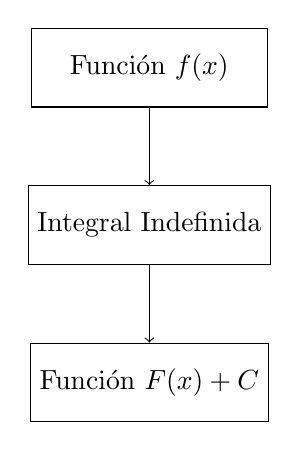
\begin{tikzpicture}[node distance=2cm]
    
    % Nodes
    \node (start) [draw, rectangle, minimum width=3cm, minimum height=1cm, text centered] {Función $f(x)$};
    \node (integral) [draw, rectangle, minimum width=3cm, minimum height=1cm, text centered, below of=start] {Integral Indefinida};
    \node (result) [draw, rectangle, minimum width=3cm, minimum height=1cm, text centered, below of=integral] {Función $F(x) + C$};
    
    % Arrows
    \draw [->] (start) -- (integral);
    \draw [->] (integral) -- (result);
    
    \end{tikzpicture}
    \end{center}

    
\begin{definition}[Integral Indefinida]
    Dada una función \( f(x) \), la integral indefinida de \( f(x) \) con respecto a \( x \) se define como:

\[
\int f(x) \, dx = F(x) + C
\]

donde \( F(x) \) es una función tal que \( \frac{dF}{dx} = f(x) \), y \( C \) es una constante arbitraria que se añade porque la derivada de una constante es cero.

\end{definition}
\begin{example}
    Si \( f(x) = 2x \), entonces:

\[
\int 2x \, dx = x^2 + C
\]

Aquí, \( F(x) = x^2 \) porque la derivada de \( x^2 \) es \( 2x \).

\end{example}
\begin{example}
    Si \( f(x) = e^x \), entonces:

\[
\int e^x \, dx = e^x + C
\]

En este caso, \( F(x) = e^x \) porque la derivada de \( e^x \) es \( e^x \).
\end{example}
\subsubsection{Propiedad de Linealidad}

La integral indefinida de una combinación lineal de funciones es igual a la combinación lineal de las integrales indefinidas de esas funciones:

\[
\int \left( a f(x) + b g(x) \right) \, dx = a \int f(x) \, dx + b \int g(x) \, dx
\]

donde \( a \) y \( b \) son constantes.

\subsubsection{Propiedad de la Integral de una Suma}

La integral indefinida de la suma de dos funciones es igual a la suma de las integrales indefinidas de esas funciones:

\[
\int \left( f(x) + g(x) \right) \, dx = \int f(x) \, dx + \int g(x) \, dx
\]

\subsubsection{Propiedad de la Integral de un Producto por una Constante}

La integral indefinida de una función multiplicada por una constante es igual a la constante multiplicada por la integral indefinida de la función:

\[
\int a f(x) \, dx = a \int f(x) \, dx
\]

\subsubsection{Propiedad de Cambio de Variable}

Si \( u = g(x) \) es una función diferenciable y \( du = g'(x) \, dx \), entonces:

\[
\int f(g(x)) \, g'(x) \, dx = \int f(u) \, du
\]

Esta propiedad permite simplificar la integración mediante un cambio de variable.

\subsubsection{Propiedad de la Integral de una Derivada}

La integral indefinida de la derivada de una función es la función original más una constante:

\[
\int \frac{dF(x)}{dx} \, dx = F(x) + C
\]

donde \( F(x) \) es una función cuya derivada es \( \frac{dF(x)}{dx} \).

\subsubsection{Integral de una Función Constante}

La integral indefinida de una función constante \( k \) es el producto de la constante por la variable \( x \) más una constante de integración:

\[
\int k \, dx = kx + C
\]

\subsubsection{Propiedad de la Integral de un Producto de Funciones}

Para la integral de un producto de funciones, se usa la técnica de integración por partes. Si \( u \) y \( v \) son funciones de \( x \), entonces:

\[
\int u \, dv = uv - \int v \, du
\]

donde \( dv \) y \( du \) son las derivadas de \( v \) y \( u \), respectivamente.

\subsubsection{Propiedad de la Integral de una Función Racional}

Para funciones racionales (cociente de dos polinomios), la integral se puede resolver mediante la descomposición en fracciones parciales. Si \( \frac{P(x)}{Q(x)} \) es una función racional, se puede expresar como una suma de fracciones más simples.

\subsubsection{Propiedad de la Integral de una Función Exponencial}

La integral de una función exponencial es:

\[
\int e^{ax} \, dx = \frac{e^{ax}}{a} + C
\]

donde \( a \) es una constante.

\subsubsection{Propiedad de la Integral de una Función Trigonométrica}

Las integrales de las funciones trigonométricas básicas son:

\[
\int \sin(x) \, dx = -\cos(x) + C
\]

\[
\int \cos(x) \, dx = \sin(x) + C
\]

\newpage
\subsection{Integrales inmediatas (uso de las tablas)}

Las integrales inmediatas son aquellas que se pueden resolver directamente usando fórmulas conocidas sin necesidad de aplicar métodos adicionales. A continuación se presentan algunas de las integrales inmediatas más comunes y sus fórmulas.

\subsubsection{Integrales de Funciones Constantes}

La integral indefinida de una constante \( k \) es:

\[
\int k \, dx = kx + C
\]

donde \( C \) es la constante de integración.

\subsubsection{Integrales de Funciones Potenciales}

La integral indefinida de \( x^n \), donde \( n \neq -1 \), es:

\[
\int x^n \, dx = \frac{x^{n+1}}{n+1} + C
\]

\subsubsection{Integrales de Funciones Exponenciales}

La integral indefinida de la función exponencial es:

\[
\int e^{ax} \, dx = \frac{e^{ax}}{a} + C
\]

donde \( a \) es una constante.

\subsubsection{Integrales de Funciones Trigonométricas}

Las integrales indefinidas de las funciones trigonométricas básicas son:

\[
\int \sin(x) \, dx = -\cos(x) + C
\]

\[
\int \cos(x) \, dx = \sin(x) + C
\]

\[
\int \sec^2(x) \, dx = \tan(x) + C
\]

\[
\int \csc^2(x) \, dx = -\cot(x) + C
\]

\subsubsection{Integrales de Funciones Logarítmicas}

La integral indefinida del logaritmo natural es:

\[
\int \frac{1}{x} \, dx = \ln |x| + C
\]


% \begin{table}[h!]
% \centering
% \begin{tabular}{|c|c|}
% \hline
% \textbf{Integral} & \textbf{Resultado} \\
% \hline
% \(\int 1 \, dx\) & \(x + C\) \\
% \(\int x \, dx\) & \(\frac{x^2}{2} + C\) \\
% \(\int x^2 \, dx\) & \(\frac{x^3}{3} + C\) \\
% \(\int e^x \, dx\) & \(e^x + C\) \\
% \(\int \sin(x) \, dx\) & \(-\cos(x) + C\) \\
% \(\int \cos(x) \, dx\) & \(\sin(x) + C\) \\
% \(\int \frac{1}{x} \, dx\) & \(\ln |x| + C\) \\
% \(\int \sec^2(x) \, dx\) & \(\tan(x) + C\) \\
% \hline
% \end{tabular}
% \caption{Tabla de Integrales Inmediatas Comunes\footnote{Asegúrate de que el resultado que obtengas de la tabla es aplicable al contexto específico del problema que estás resolviendo.}}
% \end{table}



\newpage
\subsection{Aplicaciones de las integrales indefinidas}

Las integrales indefinidas tienen muchas aplicaciones prácticas en diversas áreas de las matemáticas y las ciencias. En este documento, exploraremos algunas de las principales aplicaciones.

\subsubsection{Cálculo de Áreas Bajo la Curva}

Aunque el cálculo directo de áreas bajo la curva se realiza con integrales definidas, la integral indefinida es esencial para encontrar la función antiderivada que se evalúa en los límites de integración. Por ejemplo, para encontrar el área bajo la curva de \( f(x) = x^2 \) en el intervalo \([a, b]\), primero encontramos la integral indefinida:

\[
\int x^2 \, dx = \frac{x^3}{3} + C
\]

Luego, evaluamos esta antiderivada en \( b \) y \( a \) para encontrar el área bajo la curva.

\subsubsection{Cálculo de Volúmenes de Sólidos de Revolución}

Para calcular el volumen de un sólido de revolución, usamos la integral definida del área de secciones transversales. Por ejemplo, para un sólido generado al girar la función \( f(x) = x^2 \) alrededor del eje \( x \), el volumen \( V \) se calcula como:

\[
V = \pi \int_{a}^{b} \left[ f(x) \right]^2 \, dx
\]

Donde \( \left[ f(x) \right]^2 \) es la función del área de la sección transversal del sólido.

\subsubsection{Solución de Ecuaciones Diferenciales}

Las integrales indefinidas son cruciales para resolver ecuaciones diferenciales. Por ejemplo, para resolver la ecuación diferencial:

\[
\frac{dy}{dx} = 3x^2
\]

Integramos ambos lados con respecto a \( x \):

\[
y = \int 3x^2 \, dx = x^3 + C
\]

Aquí, \( C \) es la constante de integración que se determina mediante condiciones iniciales.

\subsubsection{Problemas de Física}

En física, las integrales indefinidas se utilizan para calcular diversas magnitudes. Por ejemplo, la distancia recorrida \( s \) cuando la velocidad \( v(t) \) es una función del tiempo \( t \) se obtiene integrando la función de velocidad:

\[
s(t) = \int v(t) \, dt
\]

Si \( v(t) = 5t \), entonces:

\[
s(t) = \int 5t \, dt = \frac{5t^2}{2} + C
\]

\subsubsection{Problemas de Ingeniería}

En ingeniería, las integrales indefinidas ayudan a encontrar el centro de masa, el momento de inercia, entre otros. Por ejemplo, el momento de inercia \( I \) de una barra uniforme de longitud \( L \) respecto a un eje que pasa por su centro se calcula usando:

\[
I = \int_{-L/2}^{L/2} x^2 \, dm
\]

donde \( dm \) es el elemento diferencial de masa.

\newpage

\section{Métodos de integración} %(20 horas) 15 clases
\newpage
\subsection{Integración por cambio de variable}
\newpage
\subsection{Integración por partes}
Para integrar productos de funciones, se desarrolla una técnica que se basa en la regla del producto para derivadas y se deriva de la fórmula general de la integración de un producto de funciones. La fórmula de integración por partes es especialmente útil cuando la integral involucra un producto de dos funciones, donde una de ellas se puede simplificar al derivarla, y la otra se puede integrar fácilmente.

\begin{proof}[Demostración de la Fómrula de Integración por Partes]
    
    Sea definida la regla del producto para la derivada de dos funciones \( u(x) \) y \( v(x) \), como:
    \begin{equation*}
    \frac{d}{dx} \left( u(x) v(x) \right) = u'(x) v(x) + u(x) v'(x)
\end{equation*}

Integrando ambos lados con respecto a \( x \), obtenemos:
\begin{equation*}
    \int \frac{d}{dx} \left( u(x) v(x) \right) \, dx = \int \left( u'(x) v(x) + u(x) v'(x) \right) \, dx
\end{equation*}
La integral del lado izquierdo es simplemente \( u(x) v(x) \):
\begin{equation*}
    u(x) v(x) = \int u'(x) v(x) \, dx + \int u(x) v'(x) \, dx
\end{equation*}
Reorganizando los términos, tenemos:
\begin{equation*}
    \int u(x) v'(x) \, dx = u(x) v(x) - \int u'(x) v(x) \, dx
\end{equation*}
Para simplificar la notación, dejamos de escribir las variables \( x \):
\begin{equation*}
    \int u \, dv = uv - \int v \, du
\end{equation*}
Donde, \( u \) es una función que derivamos para obtener \( du \), y \( dv \) es una función que integramos para obtener \( v \).
\end{proof}
\begin{definition}[Integración por partes]
    La integración por partes es una técnica derivada de la regla del producto para la derivada. La fórmula de integración por partes es:
    \begin{equation}
        \int u \, dv = uv - \int v \, du
    \end{equation}
    Donde \( u \) y \( dv \) son partes de la integral original \( \int u \, dv \).    
\end{definition}
\subsubsection{Método}
\begin{enumerate}
    \item \textbf{Identificación de \( u \) y \( dv \)}:
    \begin{itemize}
        \item Selecciona \( u \) (la función a derivar) y \( dv \) (la función a integrar).
        \item Usa la regla de LIATE (Logaritmo, Inverso trigonométrico, Algebraico, Trigonométrico, Exponencial) para seleccionar \( u \).
    \end{itemize}
    \item \textbf{Derivación de \( u \) y obtención de \( du \)}:
    \begin{itemize}
        \item Deriva \( u \) para encontrar \( du \).
    \end{itemize}
    \item \textbf{Integración de \( dv \) para encontrar \( v \)}:
    \begin{itemize}
        \item Integra \( dv \) para encontrar \( v \).
    \end{itemize}
    \item \textbf{Aplicación de la fórmula de integración por partes}:
    \begin{itemize}
        \item Sustituye \( u \), \( v \), y \( du \) en la fórmula.
        \item Simplifica y resuelve la integral restante.
    \end{itemize}
\end{enumerate}
\begin{example}
Integral con término algebraico y exponencial:
\begin{equation*}
    \int x e^x \, dx
\end{equation*}
    \textbf{Paso 1: Selección de \( u \) y \( dv \)}
    
    Siguiendo la regla LIATE:
    \begin{align*}
    u &= x \\
    dv &= e^x \, dx
    \end{align*}
\textbf{Paso 2: Derivación de \( u \) y obtención de \( du \)}
\begin{equation*}
    du = dx
\end{equation*}
    \textbf{Paso 3: Integración de \( dv \) para encontrar \( v \)}
\begin{equation*}
    v = \int e^x \, dx = e^x
\end{equation*}
    \textbf{Paso 4: Aplicación de la fórmula}
    \begin{align*}
        &\int x e^x \, dx = x e^x - \int e^x \, dx =\\
        &= \int x e^x \, dx = x e^x - e^x + C
    \end{align*}    
\end{example}
\begin{example}
Integral con término algebraico y trigonométrico:    
\begin{equation*}
    \int x \cos(x) \, dx 
\end{equation*}
    \textbf{Selección de \( u \) y \( dv \)}:
    \begin{align*}
    u &= x \\
    dv &= \cos(x) \, dx
    \end{align*}
    \textbf{Derivación de \( u \) y obtención de \( du \)}:
\begin{equation*}
    du = dx
\end{equation*}
    \textbf{Integración de \( dv \) para encontrar \( v \)}:
\begin{equation*}
    v = \int \cos(x) \, dx = \sin(x)
\end{equation*}
    \textbf{Aplicación de la fórmula}:
\begin{equation*}
    \int x \cos(x) \, dx = x \sin(x) - \int \sin(x) \, dx = x \sin(x) + \cos(x) + C
\end{equation*}
\end{example}

\begin{definition}[Método DI]
    También conocido como el método de la tabla de derivadas e integrales, es una técnica sistemática para realizar integración por partes de manera eficiente. Este método es especialmente útil cuando se tienen que realizar varias integraciones por partes consecutivas.
\end{definition}
Pasos del Método DI:
\begin{enumerate}
    \item \textbf{Identificación de \( u \) y \( dv \)}:
    \begin{itemize}
        \item Selecciona \( u \) (la función a derivar) y \( dv \) (la función a integrar).
        \item Generalmente, se sigue la regla de LIATE (Logaritmo, Inverso trigonométrico, Algebraico, Trigonométrico, Exponencial) para seleccionar \( u \).
    \end{itemize}
    \item \textbf{Construcción de la tabla DI}:
    \begin{itemize}
        \item Crea una tabla con dos columnas, una para derivadas (\( D \)) y otra para integrales (\( I \)).
        \item En la primera fila, coloca \( u \) en la columna \( D \) y \( dv \) en la columna \( I \).
    \end{itemize}
    \item \textbf{Llenado de la tabla}:
    \begin{itemize}
        \item Deriva \( u \) sucesivamente hasta que obtengas cero.
        \item Integra \( dv \) sucesivamente.
    \end{itemize}
    \item \textbf{Multiplicación diagonal}:
    \begin{itemize}
        \item Multiplica cada derivada con la integral correspondiente de la siguiente fila, alternando los signos (positivo y negativo).
    \end{itemize}
    \item \textbf{Suma de términos}:
    \begin{itemize}
        \item Suma todos los productos resultantes para obtener el resultado de la integral original.
    \end{itemize}
\end{enumerate}

\begin{example}
    
    Realizando la integración por partes de la siguiente integral usando el método DI:
\begin{equation}
    \int x e^x \, dx
\end{equation}
    
    \textbf{Paso 1: Selección de \( u \) y \( dv \)}
    
    De acuerdo a la regla LIATE, seleccionamos:
    \begin{align*}
    u &= x \\
    dv &= e^x \, dx
    \end{align*}
    
    \textbf{Paso 2: Construcción de la tabla DI}

    \[
    \begin{array}{c|c}
    D & I \\
    \hline
    x & e^x \\
    1 & e^x \\
    0 & e^x \\
    \end{array}
    \]
    
    \textbf{Paso 3: Multiplicación diagonal y suma de términos}
    
    Multiplicamos diagonalmente y alternamos los signos:
    \begin{equation*}
        \int x e^x \, dx = x \cdot e^x - \int 1 \cdot e^x \, dx
    \end{equation*}
    La primera diagonal es \( x \cdot e^x \)
    
    La segunda diagonal es \(-\int e^x \, dx\), que es \(-e^x\)
    
    Finalmente, sumamos los términos:
    \begin{equation*}
        \int x e^x \, dx = x e^x - e^x + C
    \end{equation*}
\end{example}

\begin{example}
    \textbf{Caso 1: \( \int x \cos(x) \, dx \)}
    
    \textbf{Selección de \( u \) y \( dv \)}:
    \begin{align*}
    u &= x \\
    dv &= \cos(x) \, dx
    \end{align*}
    \textbf{Tabla DI}:
\begin{equation*}
    \begin{array}{c|c}
        D & I \\
        \hline
        x & \cos(x) \\
        1 & \sin(x) \\
        0 & -\cos(x) \\
        \end{array}
\end{equation*}
    \textbf{Multiplicación diagonal y suma de términos}:
    \begin{align*}
        &\int x \cos(x) \, dx = x \sin(x) - \int \sin(x) \, dx\\ 
        &\int x \cos(x) \, dx = x \sin(x) + \cos(x) + C
    \end{align*}
\end{example}
\begin{example}
    \textbf{Caso 2: \( \int x^2 e^x \, dx \)}
    
    \textbf{Selección de \( u \) y \( dv \)}:
    
    \begin{align*}
    u &= x^2 \\
    dv &= e^x \, dx
    \end{align*}
    
    \textbf{Tabla DI}:
\begin{equation*}
    \begin{array}{c|c}
        D & I \\
        \hline
        x^2 & e^x \\
        2x & e^x \\
        2 & e^x \\
        0 & e^x \\
        \end{array}
\end{equation*}
    \textbf{Multiplicación diagonal y suma de términos}:
\begin{equation*}
    \int x^2 e^x \, dx = x^2 e^x - \int 2x e^x \, dx
\end{equation*}
Ahora, integramos \( \int 2x e^x \, dx \) usando el método DI nuevamente:
    
    \textbf{Selección de \( u \) y \( dv \)}:
    \begin{align*}
    u &= 2x \\
    dv &= e^x \, dx
    \end{align*}
    \textbf{Tabla DI}:
\begin{equation*}
    \begin{array}{c|c}
        D & I \\
        \hline
        2x & e^x \\
        2 & e^x \\
        0 & e^x \\
        \end{array}
\end{equation*}
    
    \textbf{Multiplicación diagonal y suma de términos}:
\begin{align*}
    &\int 2x e^x \, dx = 2x e^x - \int 2 e^x \, dx = 2x e^x - 2e^x + C\\
    &\int x^2 e^x \, dx = x^2 e^x - (2x e^x - 2e^x) + C = x^2 e^x - 2x e^x + 2e^x + C
\end{align*}
\end{example}    

\newpage
\subsection{Integración por fracciones parciales simples}
Esta metodología es especialmente útil cuando el grado del numerador es menor que el grado del denominador en la función racional, permitiendo una descomposición en términos lineales y cuadráticos. A través de la identificación de factores lineales y cuadráticos en el denominador, se pueden establecer integrales básicas que facilitan la resolución del problema original.
\begin{definition}[Integración por fracciones   parciales simples]
    Es una técnica utilizada para integrar funciones racionales, es decir, cocientes de polinomios. La idea es descomponer una función racional en una suma de fracciones más simples, conocidas como fracciones parciales, que pueden integrarse más fácilmente.
\end{definition}
Supongamos que tenemos una función racional de la forma:
\[
\frac{P(x)}{Q(x)}
\]
donde \( P(x) \) y \( Q(x) \) son polinomios y el grado de \( P(x) \) es menor que el grado de \( Q(x) \). Podemos descomponer esta función en una suma de fracciones parciales, cuya forma depende de los factores de \( Q(x) \).

\subsection{Tipos de Factores y Fracciones Parciales}

El proceso de descomposición en fracciones parciales se basa en la factorización del denominador del polinomio en factores más simples. Dependiendo de la forma de estos factores, la técnica se clasifica en cuatro tipos:

\begin{itemize}
    \item \textbf{Factores Lineales Simples:} Estos son factores de la forma \( (x - a) \), donde \( a \) es una constante. Para cada factor lineal simple en el denominador, se asigna una fracción parcial de la forma \( \frac{A}{x - a} \), donde \( A \) es una constante a determinar.
    \item \textbf{Factores Lineales Repetidos:} Estos son factores lineales que aparecen más de una vez, como \( (x - a)^n \). La descomposición en fracciones parciales para estos factores incluye términos como \( \frac{A_1}{x - a} + \frac{A_2}{(x - a)^2} + \cdots + \frac{A_n}{(x - a)^n} \), donde \( A_1, A_2, \ldots, A_n \) son constantes a determinar.
    \item \textbf{Factores Cuadráticos Irreducibles:} Estos son factores de la forma \( ax^2 + bx + c \), donde el discriminante \( b^2 - 4ac < 0 \) indica que el polinomio no se puede factorizar en términos reales. La descomposición en fracciones parciales para estos factores incluye fracciones de la forma \( \frac{Ax + B}{ax^2 + bx + c} \), donde \( A \) y \( B \) son constantes a determinar.
    \item \textbf{Factores Cuadráticos Irreducibles Repetidos:} Estos son factores cuadráticos que aparecen más de una vez, como \( (ax^2 + bx + c)^n \). La descomposición en fracciones parciales para estos factores incluye términos como \( \frac{A_1x + B_1}{ax^2 + bx + c} + \frac{A_2x + B_2}{(ax^2 + bx + c)^2} + \cdots + \frac{A_nx + B_n}{(ax^2 + bx + c)^n} \), donde \( A_i \) y \( B_i \) son constantes a determinar.
\end{itemize}

\subsubsection{Factores Lineales Simples}
Si \( Q(x) \) tiene un factor lineal de la forma \( (x - a) \), entonces se asigna un término de la forma:
\[
\frac{A}{x - a}
\]
\begin{proof}[Demostración de los factores lineales simples]
    Consideremos una función racional donde el numerador \( P(x) \) y el denominador \( Q(x) \) son polinomios. Supondremos que \( Q(x) \) puede ser factorizado en términos de factores lineales distintos, es decir:
\[
Q(x) = (x - a_1)(x - a_2) \cdots (x - a_n)
\]
donde \( a_1, a_2, \ldots, a_n \) son raíces distintas del polinomio \( Q(x) \). Si el grado de \( P(x) \) es menor que el grado de \( Q(x) \), podemos descomponer la función racional en fracciones parciales de la forma:
\[
\frac{P(x)}{Q(x)} = \frac{P(x)}{(x - a_1)(x - a_2) \cdots (x - a_n)} = \frac{A_1}{x - a_1} + \frac{A_2}{x - a_2} + \cdots + \frac{A_n}{x - a_n}
\]
donde \( A_1, A_2, \ldots, A_n \) son constantes que debemos determinar.

Multiplicando ambos lados de la ecuación por el denominador común \( Q(x) \) para eliminar los denominadores, obtenemos:

\[
P(x) = A_1(x - a_2)(x - a_3) \cdots (x - a_n) + A_2(x - a_1)(x - a_3) \cdots (x - a_n) + \cdots + A_n(x - a_1)(x - a_2) \cdots (x - a_{n-1})
\]

Para encontrar los coeficientes \( A_i \), podemos sustituir \( x = a_i \) en la ecuación, ya que al hacerlo, todos los términos excepto el correspondiente a \( A_i \) se anulan debido a la multiplicación por cero. Así, obtenemos:

\[
P(a_i) = A_i \prod_{\substack{j=1 \\ j \neq i}}^{n} (a_i - a_j)
\]

Despejando para \( A_i \), encontramos:

\[
A_i = \frac{P(a_i)}{\prod_{\substack{j=1 \\ j \neq i}}^{n} (a_i - a_j)}
\]
\end{proof}
\begin{example}
    Integrar la siguiente función racional:

\[
\int \frac{5}{(x - 1)(x + 3)} \, dx
\]

Descomponemos en fracciones parciales:

\[
\frac{5}{(x - 1)(x + 3)} = \frac{A}{x - 1} + \frac{B}{x + 3}
\]

Multiplicando por el denominador común y resolviendo, encontramos \( A \) y \( B \):

\[
5 = A(x + 3) + B(x - 1)
\]
se igualan los denominadores a 0:
\begin{align*}
    &x - 1 = 0\implies x = 1\\
    &x + 3 = 0\implies x = - 3
\end{align*}
Para \( x = 1 \), \( A = \frac{5}{4} \) y para \( x = -3 \), \( B = -\frac{5}{4} \). Se sustituye A y B y se integra en ambas partes:

\[
\int \frac{5}{(x - 1)(x + 3)} \, dx = \frac{5}{4} \int \frac{1}{x - 1} \, dx - \frac{5}{4} \int \frac{1}{x + 3} \, dx
\]

\[
= \frac{5}{4} \ln |x - 1| - \frac{5}{4} \ln |x + 3| + C
\]
\end{example}

\subsubsection{Factores Lineales Repetidos}
Si \( Q(x) \) tiene un factor lineal repetido de la forma \( (x - a)^n \), se asignan términos de la forma:

\[
\frac{A_1}{x - a} + \frac{A_2}{(x - a)^2} + \cdots + \frac{A_n}{(x - a)^n}
\]
\begin{proof}[Demostración de los Factores Lineales Repetidos]
    Consideremos una función racional donde el numerador \( P(x) \) y el denominador \( Q(x) \) son polinomios, y supongamos que \( Q(x) \) contiene factores lineales repetidos. Específicamente, si \( Q(x) \) tiene un factor lineal repetido de la forma \( (x - a)^n \), entonces podemos expresar la función racional como:

\[
\frac{P(x)}{Q(x)} = \frac{P(x)}{(x - a)^n \cdot R(x)}
\]

donde \( R(x) \) es un polinomio que no tiene el factor \( (x - a) \). La descomposición en fracciones parciales en este caso toma la forma:

\[
\frac{P(x)}{Q(x)} = \frac{A_1}{x - a} + \frac{A_2}{(x - a)^2} + \cdots + \frac{A_n}{(x - a)^n} + \frac{P'(x)}{R(x)}
\]

donde \( A_1, A_2, \ldots, A_n \) son constantes que debemos determinar, y \( P'(x) \) es el resto de la descomposición en fracciones parciales con respecto a \( R(x) \).

Para encontrar las constantes \( A_i \), multiplicamos ambos lados por el denominador común \( (x - a)^n \cdot R(x) \) y evaluamos en diferentes valores de \( x \) para eliminar los términos correspondientes y resolver para cada \( A_i \).

\textbf{Determinación de \( A_1, A_2, \ldots, A_n \)}:

\[
P(x) = A_1(x - a)^{n-1}R(x) + A_2(x - a)^{n-2}R(x) + \cdots + A_nR(x) + (x - a)^nP'(x)
\]

Para encontrar \( A_1 \), evaluamos en \( x = a \):

\[
P(a) = A_1 \cdot 0^{n-1}R(a) + \cdots + A_nR(a) + 0
\]

\[
A_n = \frac{P(a)}{R(a)}
\]

Para \( A_{n-1} \), derivamos la expresión de \( P(x) \) y luego evaluamos en \( x = a \):

\[
P'(a) = A_1 \cdot 0^{n-2}R(a) + \cdots + A_{n-1}R(a) + 0
\]

\[
A_{n-1} = \frac{P'(a) - A_nR'(a)}{R(a)}
\]

Continuamos este proceso hasta encontrar todos los coeficientes \( A_i \).

\end{proof}
\begin{example}
    Integrar la siguiente función racional:

\[
\int \frac{2x + 3}{(x - 2)^2} \, dx
\]

Descomponemos en fracciones parciales:

\[
\frac{2x + 3}{(x - 2)^2} = \frac{A}{x - 2} + \frac{B}{(x - 2)^2}
\]

Multiplicando por el denominador común y resolviendo, encontramos \( A \) y \( B \):

\[
2x + 3 = A(x - 2) + B
\]

Para \( x = 2 \), \( B = 7 \) y para \( A \), derivamos y evaluamos en \( x = 2 \):

\[
A = 2
\]

Entonces:

\[
\int \frac{2x + 3}{(x - 2)^2} \, dx = 2 \int \frac{1}{x - 2} \, dx + 7 \int \frac{1}{(x - 2)^2} \, dx
\]

\[
= 2 \ln |x - 2| - \frac{7}{x - 2} + C
\]
\end{example}

\subsubsection{Factores Cuadráticos Irreducibles}
Si \( Q(x) \) tiene un factor cuadrático irreducible de la forma \( (ax^2 + bx + c) \) con \( b^2 - 4ac < 0 \), se asignan términos de la forma:

\[
\frac{Ax + B}{ax^2 + bx + c}
\]

\begin{proof}[Demostración de los Factores Cuadráticos Irreducibles]
    Consideremos una función racional en la que el numerador \( P(x) \) y el denominador \( Q(x) \) son polinomios, y supongamos que \( Q(x) \) tiene un factor cuadrático irreducible de la forma \( ax^2 + bx + c \), donde \( b^2 - 4ac < 0 \). En este caso, podemos descomponer la función racional en fracciones parciales de la forma:
\[
\frac{P(x)}{Q(x)} = \frac{P(x)}{(ax^2 + bx + c)R(x)}
\]

donde \( R(x) \) es un polinomio que no contiene el factor \( ax^2 + bx + c \). La descomposición en fracciones parciales toma la forma:
\[
\frac{P(x)}{Q(x)} = \frac{Ax + B}{ax^2 + bx + c} + \frac{P'(x)}{R(x)}
\]
donde \( A \) y \( B \) son constantes que debemos determinar, y \( P'(x) \) es el resto de la descomposición con respecto a \( R(x) \).

Para encontrar \( A \) y \( B \), multiplicamos ambos lados por el denominador común \( (ax^2 + bx + c)R(x) \) para obtener:
\[
P(x) = (Ax + B)R(x) + (ax^2 + bx + c)P'(x)
\]
Comparando los coeficientes de los términos correspondientes, obtenemos un sistema de ecuaciones para \( A \) y \( B \). Esto se hace típicamente evaluando \( P(x) \) y sus derivadas, o usando valores estratégicos de \( x \) para simplificar el cálculo.

\textbf{Determinación de \( A \) y \( B \)}:

\begin{itemize}
    \item \textbf{Coeficientes de \( x^2 \)}: Igualamos los coeficientes de \( x^2 \) en ambos lados de la ecuación.
    \item \textbf{Coeficientes de \( x \)}: Igualamos los coeficientes de \( x \) en ambos lados de la ecuación.
    \item \textbf{Términos constantes}: Igualamos los términos constantes en ambos lados de la ecuación.
    
\end{itemize}
Resolviendo este sistema de ecuaciones, obtenemos los valores de \( A \) y \( B \).
\end{proof}
\begin{example}
    Integrar la siguiente función racional:

\[
\int \frac{3x + 1}{x^2 + 4} \, dx
\]

Descomponemos en fracciones parciales:

\[
\frac{3x + 1}{x^2 + 4} = \frac{Ax + B}{x^2 + 4}
\]

Multiplicando por el denominador común y resolviendo, encontramos \( A \) y \( B \):

\[
3x + 1 = A(x^2 + 4) + Bx
\]

Igualando coeficientes, encontramos:

\[
A = 0, \quad B = 3
\]

Entonces:

\[
\int \frac{3x + 1}{x^2 + 4} \, dx = \int \frac{3x}{x^2 + 4} \, dx + \int \frac{1}{x^2 + 4} \, dx
\]

La primera integral se resuelve con \( u = x^2 + 4 \) y la segunda es una forma de la función arctangente:

\[
\frac{3}{2} \ln |x^2 + 4| + \frac{1}{2} \arctan\left(\frac{x}{2}\right) + C
\]
\end{example}

\subsubsection{Factores Cuadráticos Irreducibles Repetidos}
Si \( Q(x) \) tiene un factor cuadrático irreducible repetido de la forma \( (ax^2 + bx + c)^n \), se asignan términos de la forma:

\[
\frac{A_1x + B_1}{ax^2 + bx + c} + \frac{A_2x + B_2}{(ax^2 + bx + c)^2} + \cdots + \frac{A_nx + B_n}{(ax^2 + bx + c)^n}
\]
\begin{proof}[Demostración de los Factores Cuadráticos Irreducibles Repetidos]
    Consideremos una función racional \( \frac{P(x)}{Q(x)} \) donde \( P(x) \) y \( Q(x) \) son polinomios, y el denominador \( Q(x) \) contiene un factor cuadrático irreducible repetido de la forma \( (ax^2 + bx + c)^n \), donde \( b^2 - 4ac < 0 \). La descomposición en fracciones parciales en este caso es de la forma:

    \[
    \frac{P(x)}{Q(x)} = \frac{P(x)}{(ax^2 + bx + c)^n R(x)} = \frac{A_1x + B_1}{ax^2 + bx + c} + \frac{A_2x + B_2}{(ax^2 + bx + c)^2} + \cdots + \frac{A_nx + B_n}{(ax^2 + bx + c)^n} + \frac{P'(x)}{R(x)}
    \]
    
    donde \( R(x) \) es un polinomio que no contiene el factor cuadrático irreducible \( ax^2 + bx + c \), y \( A_i \) y \( B_i \) son constantes a determinar. \( P'(x) \) es el resto de la descomposición.
    
    Para encontrar las constantes \( A_i \) y \( B_i \), multiplicamos ambos lados de la ecuación por el denominador común \( (ax^2 + bx + c)^n R(x) \) y comparamos los coeficientes de los términos correspondientes de \( P(x) \) con los de la expresión expandida.
    
    \textbf{Determinación de \( A_i \) y \( B_i \)}:
    
    Para cada \( i \) (donde \( i = 1, 2, \ldots, n \)), evaluamos la ecuación resultante en puntos estratégicos y/o derivamos con respecto a \( x \) para eliminar términos y encontrar los coeficientes \( A_i \) y \( B_i \).
    
\end{proof}
\begin{example}
    Integrar la siguiente función racional:

\[
\int \frac{2x + 3}{(x^2 + 1)^2} \, dx
\]

Descomponemos en fracciones parciales:

\[
\frac{2x + 3}{(x^2 + 1)^2} = \frac{Ax + B}{x^2 + 1} + \frac{Cx + D}{(x^2 + 1)^2}
\]

Multiplicando por el denominador común y resolviendo, encontramos \( A \), \( B \), \( C \) y \( D \):

\[
2x + 3 = (Ax + B)(x^2 + 1) + (Cx + D)
\]

Igualando coeficientes, encontramos:

\[
A = 2, \quad B = 3, \quad C = 0, \quad D = 0
\]

Entonces:

\[
\int \frac{2x + 3}{(x^2 + 1)^2} \, dx = 2 \int \frac{x}{x^2 + 1} \, dx + 3 \int \frac{1}{(x^2 + 1)^2} \, dx
\]

La primera integral se resuelve con \( u = x^2 + 1 \) y la segunda con una técnica de sustitución especial:

\[
= \ln |x^2 + 1| - \frac{x}{x^2 + 1} + C
\]

\end{example}




\subsection{Uso de las tablas de integración}

Los métodos de integración comunes incluyen cambio de variable, integración por partes y fracciones parciales. A continuación, se presenta una tabla que resume las fórmulas para cada método.

\begin{table}[h!]
    \centering
    \begin{tabular}{|c|c|}
    \hline
    \textbf{Método} & \textbf{Fórmula} \\
    \hline
    \textbf{Integración por Cambio de Variable} & \\
    \hline
    \(\int f(g(x)) \cdot g'(x) \, dx\) & \(\int f(u) \, du\) \\
    \hline
    \textbf{Integración por Partes} & \\
    \hline
    \(\int u \, dv\) & \(uv - \int v \, du\) \\
    \hline
    \textbf{Fracciones Parciales} & \\
    \hline
    \(\frac{A}{x - a}\) & \(\int \frac{A}{x - a} \, dx = A \ln |x - a| + C\) \\
    \hline
    \(\frac{A_1}{x - a} + \frac{A_2}{(x - a)^2} + \cdots + \frac{A_n}{(x - a)^n}\) & \(\int \left( \frac{A_1}{x - a} + \frac{A_2}{(x - a)^2} + \cdots + \frac{A_n}{(x - a)^n} \right) \, dx\) \\
    \hline
    \(\frac{Ax + B}{x^2 + bx + c}\) & \(\int \frac{Ax + B}{x^2 + bx + c} \, dx\) \\
    \hline
    \(\frac{Ax + B}{x^2 + bx + c} + \frac{C_1x + D_1}{(x^2 + bx + c)^2} + \cdots + \frac{E}{(x^2 + bx + c)^n}\) & \(\int \frac{Ax + B}{x^2 + bx + c} \, dx + \int \frac{C_1x + D_1}{(x^2 + bx + c)^2} \, dx + \cdots\) \\
    \hline
    \end{tabular}
    \caption{Tabla de Fórmulas de Integración}
    \end{table}

\subsection{Integrales trigonométricas}
Las integrales trigonométricas son una categoría importante de integrales que involucran funciones trigonométricas como seno, coseno, tangente y sus recíprocas. Estas integrales aparecen con frecuencia en problemas de física e ingeniería, así como en diversos campos de las matemáticas aplicadas. Resolver integrales trigonométricas requiere el uso de identidades trigonométricas y técnicas de integración específicas para simplificar las expresiones y encontrar la solución.

Las integrales trigonométricas se pueden clasificar en varias categorías, tales como:

\begin{itemize}
    \item \textbf{Integrales de funciones trigonométricas simples:} Estas incluyen integrales de funciones como \( \sin x \), \( \cos x \), \( \tan x \), etc.
    \item \textbf{Integrales de productos de funciones trigonométricas:} Estas implican productos de funciones trigonométricas, como \( \sin x \cdot \cos x \).
    \item \textbf{Integrales que involucran funciones trigonométricas elevadas a una potencia:} Estas son integrales que involucran funciones trigonométricas elevadas a una potencia, como \( \sin^2 x \) o \( \cos^3 x \).
    \item \textbf{Integrales que involucran funciones trigonométricas en fracciones:} Estas implican fracciones donde el numerador y/o el denominador es una función trigonométrica, como \( \frac{\sin x}{\cos x} \).
\end{itemize}

Para resolver integrales trigonométricas, a menudo se utilizan identidades trigonométricas para simplificar la integral, así como métodos de sustitución y técnicas de integración por partes.

\subsubsection{Integrales de Funciones Trigonométricas Básicas}

Estas integrales son las más directas y se basan en las fórmulas estándar de integrales de funciones trigonométricas.

\textbf{Ejemplos:}

\begin{itemize}
  \item \(\int \sin(x) \, dx = -\cos(x) + C\)
  \item \(\int \cos(x) \, dx = \sin(x) + C\)
  \item \(\int \sec^2(x) \, dx = \tan(x) + C\)
  \item \(\int \csc^2(x) \, dx = -\cot(x) + C\)
\end{itemize}

\subsubsection{Integrales de Productos de Funciones Trigonométricas}

Para productos de funciones trigonométricas, se pueden usar identidades trigonométricas para simplificar la integral antes de resolverla.

\begin{example}
    Para la integral:

\[
\int \sin(x) \cos(x) \, dx
\]

Usamos la identidad \(\sin(2x) = 2 \sin(x) \cos(x)\):

\[
\sin(x) \cos(x) = \frac{1}{2} \sin(2x)
\]

Entonces:

\[
\int \sin(x) \cos(x) \, dx = \frac{1}{2} \int \sin(2x) \, dx
\]

\[
\int \sin(2x) \, dx = -\frac{1}{2} \cos(2x) + C
\]

Por lo tanto:

\[
\int \sin(x) \cos(x) \, dx = -\frac{1}{4} \cos(2x) + C
\]
\end{example}

\subsubsection{Integrales de Funciones Trigonométricas Elevadas a Potencias}

Para integrales de funciones trigonométricas elevadas a potencias, se pueden usar identidades trigonométricas y técnicas de reducción de potencias.

\begin{example}
    
Para la integral:

\[
\int \sin^2(x) \, dx
\]

Usamos la identidad \(\sin^2(x) = \frac{1 - \cos(2x)}{2}\):

\[
\int \sin^2(x) \, dx = \int \frac{1 - \cos(2x)}{2} \, dx
\]

\[
= \frac{1}{2} \int 1 \, dx - \frac{1}{2} \int \cos(2x) \, dx
\]

\[
= \frac{x}{2} - \frac{1}{4} \sin(2x) + C
\]
\end{example}

\subsubsection{Integrales de Funciones Trigonométricas en Combinación con Polinomios}

Para integrales que combinan funciones trigonométricas y polinomios, es útil usar la técnica de integración por partes o sustituciones adecuadas.

\begin{example}
    Para la integral:

\[
\int x \cos(x) \, dx
\]

Usamos integración por partes. Elegimos \(u = x\) y \(dv = \cos(x) \, dx\):

\[
du = dx \quad \text{y} \quad v = \sin(x)
\]

Aplicamos la fórmula de integración por partes:

\[
\int x \cos(x) \, dx = x \sin(x) - \int \sin(x) \, dx
\]

\[
= x \sin(x) + \cos(x) + C
\]
\end{example}

\subsection{Integración por sustitución trigonométrica}

La integración por sustitución trigonométrica es una técnica utilizada para resolver integrales que involucran raíces cuadradas de expresiones cuadráticas. Esta técnica es especialmente útil para integrales de la forma:

\[
\int \frac{1}{\sqrt{a^2 - x^2}} \, dx
\]

\[
\int \frac{1}{\sqrt{x^2 - a^2}} \, dx
\]

\[
\int \frac{1}{\sqrt{x^2 + a^2}} \, dx
\]

donde \( a \) es una constante y \( x \) es la variable de integración.

Para integrar estas funciones, utilizamos sustituciones basadas en identidades trigonométricas. Los tres casos comunes son:

\begin{itemize}
  \item \textbf{Caso 1:} \( x = a \sin(\theta) \)
  \item \textbf{Caso 2:} \( x = a \cos(\theta) \)
  \item \textbf{Caso 3:} \( x = a \tan(\theta) \)
\end{itemize}

Donde cada caso corresponde a una forma diferente de la expresión bajo la raíz cuadrada.


\subsubsection{Caso 1: \( x = a \sin(\theta) \)}

Para integrales de la forma:

\[
\int \frac{1}{\sqrt{a^2 - x^2}} \, dx
\]

Utilizamos la sustitución \( x = a \sin(\theta) \). Entonces, \( dx = a \cos(\theta) \, d\theta \) y la integral se transforma en:

\[
\int \frac{a \cos(\theta) \, d\theta}{\sqrt{a^2 - a^2 \sin^2(\theta)}}
\]

Simplificamos usando la identidad \(\cos^2(\theta) = 1 - \sin^2(\theta)\):

\[
\sqrt{a^2 - a^2 \sin^2(\theta)} = a \cos(\theta)
\]

Por lo tanto:

\[
\int \frac{a \cos(\theta) \, d\theta}{a \cos(\theta)} = \int d\theta = \theta + C
\]

Regresamos a la variable original \( x \) usando \(\theta = \arcsin\left(\frac{x}{a}\right)\):

\[
\theta = \arcsin\left(\frac{x}{a}\right) \quad \text{entonces} \quad \int \frac{1}{\sqrt{a^2 - x^2}} \, dx = \arcsin\left(\frac{x}{a}\right) + C
\]

\subsubsection{Caso 2: \( x = a \cos(\theta) \)}

Para integrales de la forma:

\[
\int \frac{1}{\sqrt{x^2 - a^2}} \, dx
\]

Utilizamos la sustitución \( x = a \cos(\theta) \). Entonces, \( dx = -a \sin(\theta) \, d\theta \) y la integral se transforma en:

\[
\int \frac{-a \sin(\theta) \, d\theta}{\sqrt{a^2 \cos^2(\theta) - a^2}}
\]

Simplificamos usando la identidad \(\sin^2(\theta) = 1 - \cos^2(\theta)\):

\[
\sqrt{a^2 \cos^2(\theta) - a^2} = a \sqrt{\cos^2(\theta) - 1} = a \sqrt{-\sin^2(\theta)} = a \sin(\theta)
\]

Por lo tanto:

\[
\int \frac{-a \sin(\theta) \, d\theta}{a \sin(\theta)} = - \int d\theta = -\theta + C
\]

Regresamos a la variable original \( x \) usando \(\theta = \arccos\left(\frac{x}{a}\right)\):

\[
\theta = \arccos\left(\frac{x}{a}\right) \quad \text{entonces} \quad \int \frac{1}{\sqrt{x^2 - a^2}} \, dx = -\arccos\left(\frac{x}{a}\right) + C
\]

\subsubsection{Caso 3: \( x = a \tan(\theta) \)}

Para integrales de la forma:

\[
\int \frac{1}{\sqrt{x^2 + a^2}} \, dx
\]

Utilizamos la sustitución \( x = a \tan(\theta) \). Entonces, \( dx = a \sec^2(\theta) \, d\theta \) y la integral se transforma en:

\[
\int \frac{a \sec^2(\theta) \, d\theta}{\sqrt{a^2 \tan^2(\theta) + a^2}}
\]

Simplificamos usando la identidad \(\sec^2(\theta) = 1 + \tan^2(\theta)\):

\[
\sqrt{a^2 \tan^2(\theta) + a^2} = a \sec(\theta)
\]

Por lo tanto:

\[
\int \frac{a \sec^2(\theta) \, d\theta}{a \sec(\theta)} = \int \sec(\theta) \, d\theta
\]

La integral de \(\sec(\theta)\) es conocida:

\[
\int \sec(\theta) \, d\theta = \ln|\sec(\theta) + \tan(\theta)| + C
\]

Regresamos a la variable original \( x \) usando \( \sec(\theta) = \sqrt{1 + \tan^2(\theta)} = \sqrt{1 + \left(\frac{x}{a}\right)^2} \) y \( \tan(\theta) = \frac{x}{a} \):

\[
\int \frac{1}{\sqrt{x^2 + a^2}} \, dx = \ln \left| \frac{x + \sqrt{x^2 + a^2}}{a} \right| + C
\]



\newpage
%%%%%%%%%%%%%%%%%%%%%%%%%%%%%%%%%%%%%%%%%%%%%%%%%%%%%%%%%%%%%%%%%%%%%%%%%%%%%%%%%%%%%%%%%%%%%%%%
%%%%%%%%%%%%%%%%%%%%%%%%%%%%%%%%%%%%%%%%%%%%%%%%%%%%%%%%%%%%%%%%%%%%%%%%%%%%%%%%%%%%%%%%%%%%%%%%
%%%%%%%%%%%%%%%%%%%%%%%%%%%%%%%%%%%%%%%%%%%%%%%%%%%%%%%%%%%%%%%%%%%%%%%%%%%%%%%%%%%%%%%%%%%%%%%%
%%%%%%%%%%%%%%%%%%%%%%%%%%%%%%%%%%%%%%%%%%%%%%%%%%%%%%%%%%%%%%%%%%%%%%%%%%%%%%%%%%%%%%%%%%%%%%%%
%%%%%%%%%%%%%%%%%%%%%%%%%%%%%%%%%%%%%%%%%%%%%%%%%%%%%%%%%%%%%%%%%%%%%%%%%%%%%%%%%%%%%%%%%%%%%%%%
%%%%%%%%%%%%%%%%%%%%%%%%%%%%%%%%%%%%%%%%%%%%%%%%%%%%%%%%%%%%%%%%%%%%%%%%%%%%%%%%%%%%%%%%%%%%%%%%
%%%%%%%%%%%%%%%%%%%%%%%%%%%%%%%%%%%%%%%%%%%%%%%%%%%%%%%%%%%%%%%%%%%%%%%%%%%%%%%%%%%%%%%%%%%%%%%%
%%%%%%%%%%%%%%%%%%%%%%%%%%%%%%%%%%%%%%%%%%%%%%%%%%%%%%%%%%%%%%%%%%%%%%%%%%%%%%%%%%%%%%%%%%%%%%%%
%%%%%%%%%%%%%%%%%%%%%%%%%%%%%%%%%%%%%%%%%%%%%%%%%%%%%%%%%%%%%%%%%%%%%%%%%%%%%%%%%%%%%%%%%%%%%%%%
%%%%%%%%%%%%%%%%%%%%%%%%%%%%%%%%%%%%%%%%%%%%%%%%%%%%%%%%%%%%%%%%%%%%%%%%%%%%%%%%%%%%%%%%%%%%%%%%
%%%%%%%%%%%%%%%%%%%%%%%%%%%%%%%%%%%%%%%%%%%%%%%%%%%%%%%%%%%%%%%%%%%%%%%%%%%%%%%%%%%%%%%%%%%%%%%%
%%%%%%%%%%%%%%%%%%%%%%%%%%%%%%%%%%%%%%%%%%%%%%%%%%%%%%%%%%%%%%%%%%%%%%%%%%%%%%%%%%%%%%%%%%%%%%%%

\section{La integral definida}%(20 horas) 15 clases

La integral definida representa el área bajo la curva de una función en un intervalo específico. Dada una función \( f(x) \) y un intervalo \([a, b]\), la integral definida de \( f(x) \) desde \( a \) hasta \( b \) se denota como:
\begin{equation*}
    \int_{a}^{b} f(x) \, dx
\end{equation*}
El valor de esta integral se calcula como la diferencia entre las antiderivadas evaluadas en los límites superior e inferior:
\begin{equation}
    \int_{a}^{b} f(x) \, dx = F(b) - F(a)
\end{equation}

Donde \( F(x) \) es una función antiderivada de \( f(x) \), es decir, \( F'(x) = f(x) \).

La integral definida de una función \( f \) en el intervalo \([a, b]\) se define formalmente como el límite de la suma de Riemann de \( f \) en ese intervalo a medida que el número de particiones tiende al infinito. 

\begin{definition}[Suma de Riemann]
    Sea \( f \) una función definida en el intervalo cerrado \([a, b]\). Dividimos el intervalo \([a, b]\) en \( n \) subintervalos de igual longitud \(\Delta x\):

\[
\Delta x = \frac{b - a}{n}
\]

Sea \( x_i^* \) un punto arbitrario en el \( i \)-ésimo subintervalo \([x_{i-1}, x_i]\), donde \( x_i = a + i \Delta x \) para \( i = 1, 2, \ldots, n \). La suma de Riemann para \( f \) en esta partición es:

\[
S_n = \sum_{i=1}^{n} f(x_i^*) \Delta x
\]

La integral definida de \( f \) desde \( a \) hasta \( b \) está definida como el límite de esta suma de Riemann cuando el número de particiones \( n \) tiende al infinito:

\[
\int_{a}^{b} f(x) \, dx = \lim_{n \to \infty} \sum_{i=1}^{n} f(x_i^*) \Delta x
\]

Donde el límite existe y es independiente de la elección de los puntos \( x_i^* \) en los subintervalos.
\end{definition}

\begin{multicols}{2}
\begin{center}
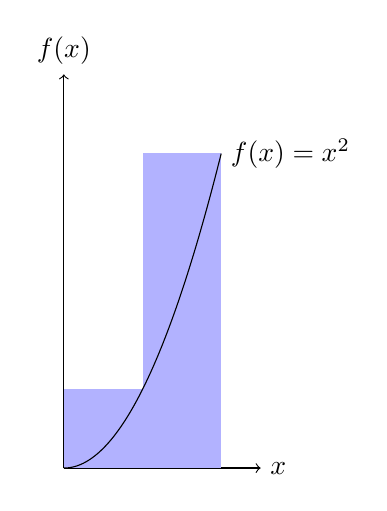
\begin{tikzpicture}
    % Dibuja los ejes
    \draw[->] (0,0) -- (2.5,0) node[right] {$x$};
    \draw[->] (0,0) -- (0,5) node[above] {$f(x)$};
    
    % Dibuja las barras de la suma de Riemann
    \fill[blue!30] (0,0) rectangle (1,1);
    \fill[blue!30] (1,0) rectangle (2,4);
    
        % Dibuja la función f(x) = x^2
        \draw[domain=0:2, smooth, variable=\x, samples=100] plot ({\x}, {\x*\x}) node[right] {$f(x) = x^2$};
\end{tikzpicture}
\end{center}

\begin{center}
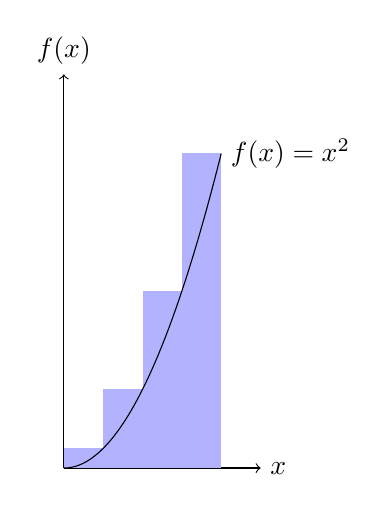
\begin{tikzpicture}
    % Dibuja los ejes
    \draw[->] (0,0) -- (2.5,0) node[right] {$x$};
    \draw[->] (0,0) -- (0,5) node[above] {$f(x)$};
    
    % Dibuja las barras de la suma de Riemann
    \fill[blue!30] (0,0) rectangle (0.5,0.25);
    \fill[blue!30] (0.5,0) rectangle (1,1);
    \fill[blue!30] (1,0) rectangle (1.5,2.25);
    \fill[blue!30] (1.5,0) rectangle (2,4);
    
        % Dibuja la función f(x) = x^2
        \draw[domain=0:2, smooth, variable=\x, samples=100] plot ({\x}, {\x*\x}) node[right] {$f(x) = x^2$};
\end{tikzpicture}
\end{center}

\begin{center}
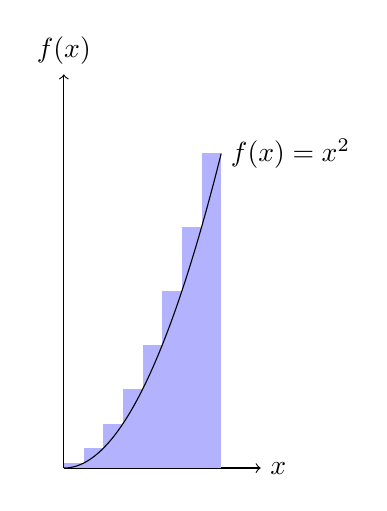
\begin{tikzpicture}
    % Dibuja los ejes
    \draw[->] (0,0) -- (2.5,0) node[right] {$x$};
    \draw[->] (0,0) -- (0,5) node[above] {$f(x)$};
    
    % Dibuja las barras de la suma de Riemann
    \fill[blue!30] (0,0) rectangle (0.25,0.0625);
    \fill[blue!30] (0.25,0) rectangle (0.5,0.25);
    \fill[blue!30] (0.5,0) rectangle (0.75,0.5625);
    \fill[blue!30] (0.75,0) rectangle (1,1);
    \fill[blue!30] (1,0) rectangle (1.25,1.5625);
    \fill[blue!30] (1.25,0) rectangle (1.5,2.25);
    \fill[blue!30] (1.5,0) rectangle (1.75,3.0625);
    \fill[blue!30] (1.75,0) rectangle (2,4);
    
        % Dibuja la función f(x) = x^2
        \draw[domain=0:2, smooth, variable=\x, samples=100] plot ({\x}, {\x*\x}) node[right] {$f(x) = x^2$};
\end{tikzpicture}
\end{center}

\begin{center}
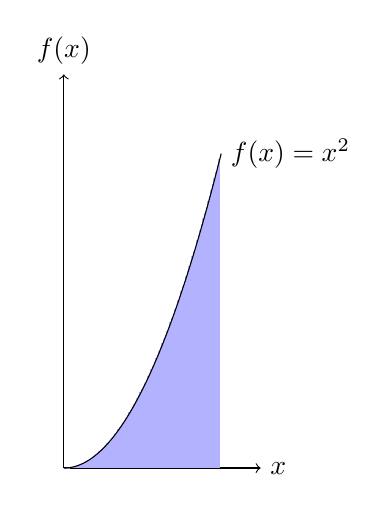
\begin{tikzpicture}
    % Dibuja los ejes
    \draw[->] (0,0) -- (2.5,0) node[right] {$x$};
    \draw[->] (0,0) -- (0,5) node[above] {$f(x)$};
    
    % Dibuja las barras de la suma de Riemann
    \foreach \i in {0,0.02,...,1.98}
    \fill[blue!30] (\i,0) rectangle (\i+0.02,{(\i+0.02)^2});
    
        % Dibuja la función f(x) = x^2
        \draw[domain=0:2, smooth, variable=\x, samples=100] plot ({\x}, {\x*\x}) node[right] {$f(x) = x^2$};
\end{tikzpicture}
\end{center}
\end{multicols}

Dada una función \( f \) continua en el intervalo cerrado \([a, b]\), la integral definida \(\int_{a}^{b} f(x) \, dx\) posee las siguientes propiedades:

\subsection{La integral definida. Propiedades.}

\subsubsection{1. Linealidad}

Para funciones \( f(x) \) y \( g(x) \) y constantes \( c_1 \) y \( c_2 \):

\[
\int_{a}^{b} \left(c_1 f(x) + c_2 g(x)\right) \, dx = c_1 \int_{a}^{b} f(x) \, dx + c_2 \int_{a}^{b} g(x) \, dx
\]

Esta propiedad indica que la integral de una combinación lineal de funciones es la combinación lineal de las integrales de las funciones.

\subsubsection{2. Adición de Intervalos}

Si \( a \leq c \leq b \), entonces:

\[
\int_{a}^{b} f(x) \, dx = \int_{a}^{c} f(x) \, dx + \int_{c}^{b} f(x) \, dx
\]

Esta propiedad permite dividir el intervalo de integración en subintervalos.

\subsubsection{3. Cambio de Orden de los Límites}

Si \( a \leq b \), entonces:

\[
\int_{a}^{b} f(x) \, dx = - \int_{b}^{a} f(x) \, dx
\]

Esta propiedad muestra que cambiar el orden de los límites cambia el signo de la integral.

\subsubsection{4. Integral de una Constante}

Para una constante \( c \):

\[
\int_{a}^{b} c \, dx = c (b - a)
\]

Esta propiedad indica que la integral de una constante sobre un intervalo es simplemente la constante multiplicada por la longitud del intervalo.

\subsubsection{5. Integral de una Función Nula}

Para \( f(x) = 0 \):

\[
\int_{a}^{b} 0 \, dx = 0
\]

Esta propiedad indica que la integral de la función nula es cero.

\subsubsection{6. Integral de una Función Par y Función Impar en Intervalos Simétricos}

Si \( f(x) \) es una función impar, entonces:

\[
\int_{-a}^{a} f(x) \, dx = 0
\]

Si \( f(x) \) es una función par, entonces:

\[
\int_{-a}^{a} f(x) \, dx = 2 \int_{0}^{a} f(x) \, dx
\]

Estas propiedades ayudan a simplificar el cálculo de integrales cuando se trabaja con funciones pares o impares en intervalos simétricos.

\subsubsection{7. Teorema Fundamental del Cálculo}

Si \( F \) es una antiderivada de \( f \) en el intervalo \([a, b]\), entonces:

\[
\int_{a}^{b} f(x) \, dx = F(b) - F(a)
\]

Este teorema conecta la integral definida con el concepto de antiderivada, proporcionando una manera directa de calcular la integral.





\subsection{Interpretaciones geométrica y física.}
La integral definida \(\int_{a}^{b} f(x) \, dx\) representa el área neta bajo la curva de \( f(x) \) en el intervalo \([a, b]\), teniendo en cuenta que el área sobre el eje \( x \) es positiva y el área bajo el eje \( x \) es negativa.

La integral definida representa el área neta bajo la curva de \( f(x) \) desde \( x = a \) hasta \( x = b \). Esta área puede ser positiva o negativa dependiendo del signo de \( f(x) \) en el intervalo. 

\subsubsection{Cálculo del Área}

Para calcular el área bajo la curva, podemos utilizar el siguiente proceso:

\begin{itemize}
    \item Si \( f(x) \geq 0 \) en \([a, b]\), el área es simplemente la integral de \( f(x) \) en ese intervalo.
    \item Si \( f(x) \leq 0 \) en \([a, b]\), el área bajo la curva es negativa y la integral representa el valor absoluto del área bajo la curva.
    \item Si \( f(x) \) cruza el eje \( x \) en el intervalo \([a, b]\), la integral considera las áreas positivas y negativas y calcula el área neta.
\end{itemize}

\begin{example}
    Consideremos la integral definida de \( f(x) = \ln(x) \) en el intervalo \([a, b]\):

\[
\int_{a}^{b} \ln(x) \, dx
\]

Para resolver esta integral, utilizamos el método de integración por partes:

\[
\int \ln(x) \, dx = x \ln(x) - \int x \cdot \frac{1}{x} \, dx = x \ln(x) - \int 1 \, dx = x \ln(x) - x + C
\]

Entonces:

\[
\int_{a}^{b} \ln(x) \, dx = \left[ x \ln(x) - x \right]_{a}^{b} = \left( b \ln(b) - b \right) - \left( a \ln(a) - a \right)
\]

Simplificando, obtenemos:

\[
\int_{a}^{b} \ln(x) \, dx = b \ln(b) - b - a \ln(a) + a
\]
\end{example}

Esta integral se interpreta geométricamente como el área neta entre la gráfica de la función \( f(x) \) y el eje \( x \), desde \( x = a \) hasta \( x = b \). 

La integral definida tiene varias aplicaciones importantes, como el cálculo de áreas bajo curvas, la determinación de volúmenes de sólidos de revolución, y el cálculo de longitudes de curvas.

\section{Gráfico Ilustrativo}

El siguiente gráfico muestra la interpretación geométrica de la integral definida. Consideremos la función \( f(x) = \ln{x}\) en el intervalo \([a, b]\). El área bajo la curva de \( f(x) \) desde \( x = a \) hasta \( x = b \) es lo que representa la integral definida.

    \begin{center}
        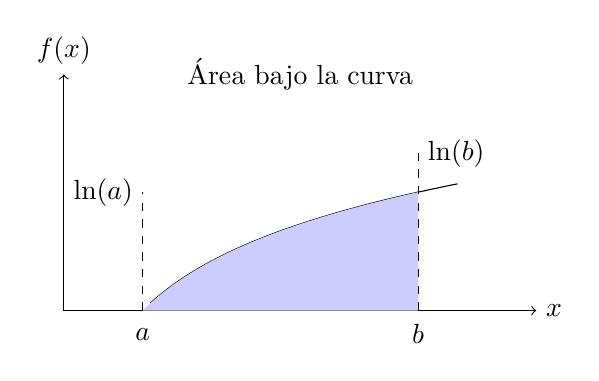
\begin{tikzpicture}
            % Dibuja los ejes
            \draw[->] (0,0) -- (6,0) node[right] {$x$};
            \draw[->] (0,0) -- (0,3) node[above] {$f(x)$};
        
            % Dibuja la función f(x) = ln(x)
            \draw[domain=1.1:5, smooth, variable=\x, samples=100] plot ({\x}, {ln(\x)});
        
            % Dibuja el área bajo la curva
            \fill[blue!20] (1,0) -- plot[domain=1.1:4.5] (\x, {ln(\x)}) -- (4.5,0) -- cycle;
        
            % Etiquetas
            \node at (3, 3) {Área bajo la curva};
            \node at (1, -0.3) {$a$};
            \node at (4.5, -0.3) {$b$};
            \draw[dashed] (1,0) -- (1,1.5) node[left] {$\ln(a)$};
            \draw[dashed] (4.5,0) -- (4.5,2) node[right] {$\ln(b)$};
        \end{tikzpicture}
\end{center}

En el gráfico anterior:

\begin{itemize}
    \item La función \( f(x) \) está representada por la curva azul.
    \item El área sombreada en azul representa la integral definida de \( f(x) \) desde \( x = a \) hasta \( x = b \).
    \item Esta área se calcula como:

    \[
    \int_{a}^{b} f(x) \, dx
    \]
\end{itemize}

La integral definida puede ser positiva, negativa o cero, dependiendo de si la función \( f(x) \) está por encima o por debajo del eje \( x \) en el intervalo \([a, b]\).

A continuación se muestran tres casos que ilustran cómo el signo de la función \( f(x) \) afecta la integral definida.


\subsubsection{Caso 1: Área por encima del eje x}

En este caso, la función \( f(x) \) es positiva en el intervalo \([a, b]\). La integral definida representa el área bajo la curva que está por encima del eje \( x \).

\begin{center}
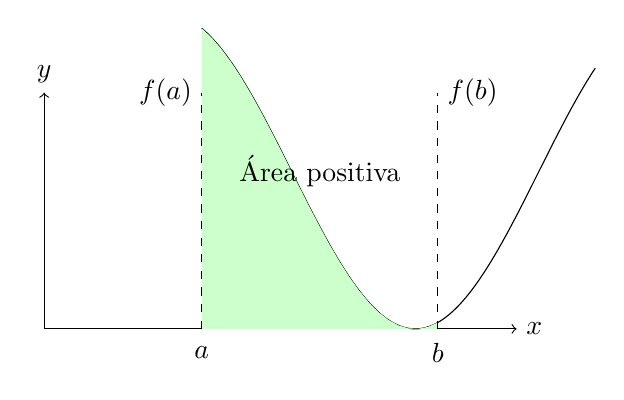
\begin{tikzpicture}
    % Dibuja los ejes
    \draw[->] (0,0) -- (6,0) node[right] {$x$};
    \draw[->] (0,0) -- (0,3) node[above] {$y$};

    % Dibuja la función f(x)
    \draw[domain=2:7, smooth, variable=\x, samples=100] plot ({\x}, {2*sin(\x r) + 2});

    % Dibuja el área bajo la curva
    \fill[green!20] (2,0) -- plot[domain=2:5] (\x, {2*sin(\x r) + 2}) -- (5,0) -- cycle;

    % Etiquetas
    \node at (3.5, 2) {Área positiva};
    \node at (2, -0.3) {$a$};
    \node at (5, -0.3) {$b$};
    \draw[dashed] (2,0) -- (2,3) node[left] {$f(a)$};
    \draw[dashed] (5,0) -- (5,3) node[right] {$f(b)$};
\end{tikzpicture}
\end{center}

\subsubsection{Caso 2: Área por debajo del eje x}

En este caso, la función \( f(x) \) es negativa en el intervalo \([a, b]\). La integral definida representa el área bajo la curva que está por debajo del eje \( x \).

\begin{center}
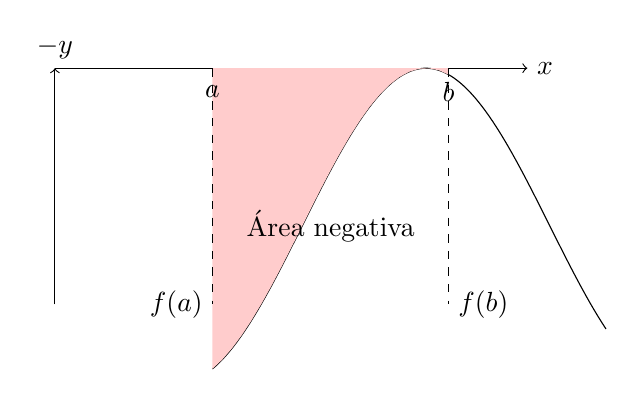
\begin{tikzpicture}
    % Dibuja los ejes
    \draw[->] (0,0) -- (6,0) node[right] {$x$};
    \draw[->] (0,-3) -- (0,0) node[above] {$-y$};

    % Dibuja la función f(x)
    \draw[domain=2:7, smooth, variable=\x, samples=100] plot ({\x}, {-2*sin(\x r) - 2});

    % Dibuja el área bajo la curva
    \fill[red!20] (2,0) -- plot[domain=2:5] (\x, {-2*sin(\x r) - 2}) -- (5,0) -- cycle;

    % Etiquetas
    \node at (3.5, -2) {Área negativa};
    \node at (2, -0.3) {$a$};
    \node at (5, -0.3) {$b$};
    \draw[dashed] (2,0) -- (2,-3) node[left] {$f(a)$};
    \draw[dashed] (5,0) -- (5,-3) node[right] {$f(b)$};
\end{tikzpicture}
\end{center}

\subsubsection{Caso 3: Función que cruza el eje x}

En este caso, la función \( f(x) \) cruza el eje \( x \) en el intervalo \([a, b]\). La integral definida considera el área neta, es decir, el área positiva y negativa.

\begin{center}
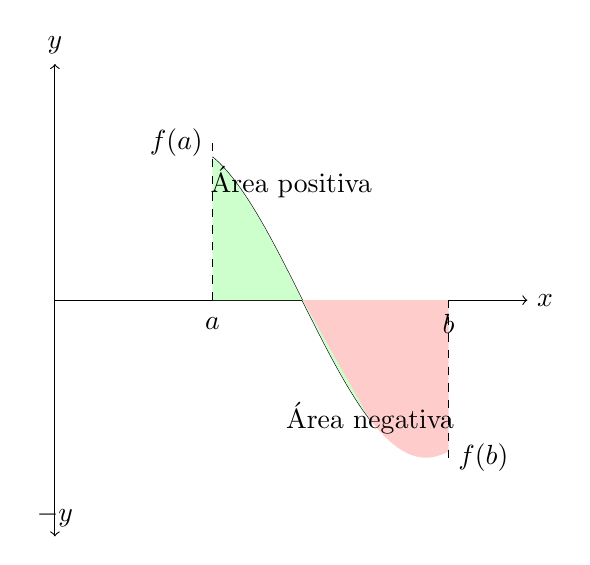
\begin{tikzpicture}
    % Dibuja los ejes
    \draw[->] (0,0) -- (6,0) node[right] {$x$};
    \draw[->] (0,-3) -- (0,3) node[above] {$y$};
    \draw[->] (0,-1) -- (0,-3) node[above] {$-y$};

    % Dibuja la función f(x)
    \draw[domain=2:4, smooth, variable=\x, samples=100] plot ({\x}, {2*sin(\x r)});

    % Dibuja el área positiva y negativa
    \fill[green!20] (2,0) -- plot[domain=2:4] (\x, {2*sin(\x r)}) -- (4,0) -- cycle;
    \fill[red!20] (3.15,0) -- plot[domain=4:5] (\x, {2*sin(\x r)}) -- (5,0) -- cycle;

    % Etiquetas
    \node at (3, 1.5) {Área positiva};
    \node at (4, -1.5) {Área negativa};
    \node at (2, -0.3) {$a$};
    \node at (5, -0.3) {$b$};
    \draw[dashed] (2,0) -- (2,2) node[left] {$f(a)$};
    \draw[dashed] (5,0) -- (5,-2) node[right] {$f(b)$};
\end{tikzpicture}
\end{center}

\subsection{Teorema Fundamental del Cálculo}

El Teorema Fundamental del Cálculo conecta el concepto de derivada con el de integral. Se divide en dos partes principales:

\subsubsection{Primera Parte}
Si \( f \) es continua en el intervalo \([a, b]\), y \( F \) es una función tal que \( F'(x) = f(x) \) para todo \( x \) en \([a, b]\), entonces:

\[
\int_a^b f(x) \, dx = F(b) - F(a)
\]

Esto significa que la integral definida de una función en un intervalo puede calcularse usando cualquier antiderivada de la función.

\subsubsection{Segunda Parte}
Si \( f \) es una función continua en un intervalo abierto \( I \) y \( a \) es un punto en \( I \), entonces la función \( F \) definida por:

\[
F(x) = \int_a^x f(t) \, dt
\]

para todo \( x \) en \( I \), es continua en \( I \), diferenciable en el interior de \( I \), y \( F'(x) = f(x) \).

\section{Ejemplo}

Consideremos la función \( f(x) = 3x^2 \). Queremos encontrar el área bajo la curva de \( f(x) \) desde \( x = 1 \) hasta \( x = 3 \).

Primero, encontramos una antiderivada de \( f(x) \). Una antiderivada de \( 3x^2 \) es \( F(x) = x^3 \) (ya que la derivada de \( x^3 \) es \( 3x^2 \)).

Aplicando el Teorema Fundamental del Cálculo, obtenemos:

\[
\int_1^3 3x^2 \, dx = F(3) - F(1) = 3^3 - 1^3 = 27 - 1 = 26
\]

Por lo tanto, el área bajo la curva de \( f(x) = 3x^2 \) desde \( x = 1 \) hasta \( x = 3 \) es 26 unidades cuadradas.

\section{Gráfico del Ejemplo}

\begin{center}
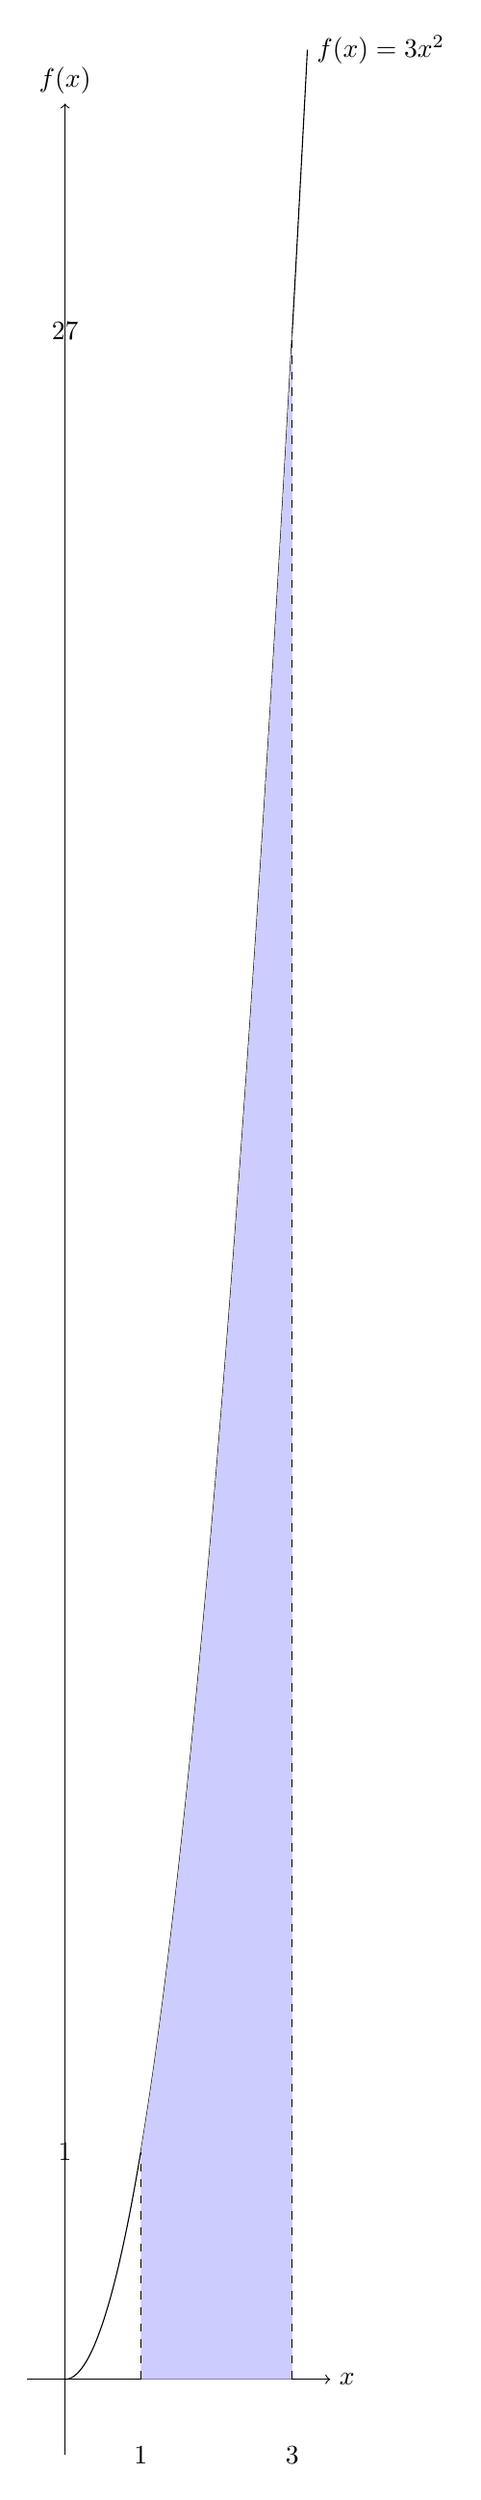
\begin{tikzpicture}
    % Dibuja los ejes
    \draw[->] (-0.5,0) -- (3.5,0) node[right] {$x$};
    \draw[->] (0,-1) -- (0,30) node[above] {$f(x)$};

    % Dibuja la función f(x) = 3x^2
    \draw[domain=0:3.2, smooth, variable=\x, samples=100] plot ({\x}, {3*\x*\x}) node[right] {$f(x) = 3x^2$};

    % Dibuja la integral definida
    \fill[blue!20] (1,0) -- plot[domain=1:3, smooth] (\x, {3*\x*\x}) -- (3,0) -- cycle;

    % Etiquetas
    \node at (1,-1) {$1$};
    \node at (3,-1) {$3$};
    \node at (0,27) {$27$};
    \node at (0,3) {$1$};

    % Líneas verticales en x=1 y x=3
    \draw[dashed] (1,0) -- (1,3);
    \draw[dashed] (3,0) -- (3,27);
\end{tikzpicture}
\end{center}

\subsection{Aplicaciones de la integral definida}
La integral definida tiene numerosas aplicaciones en matemáticas y ciencias. A continuación, se presentan ejemplos de problemas prácticos que ilustran diferentes usos de la integral definida, junto con sus soluciones y gráficos.



\subsubsection{Área bajo una curva}
\begin{example}
    \textbf{Problema:} Calcular el área bajo la curva \( f(x) = 4 - x^2 \) en el intervalo \([0, 2]\).
    
    \textbf{Solución:}
    \[
    \text{Área} = \int_0^2 (4 - x^2) \, dx = \left[ 4x - \frac{x^3}{3} \right]_0^2 = (8 - \frac{8}{3}) - (0 - 0) = \frac{16}{3}
    \]
    
    \begin{center}
    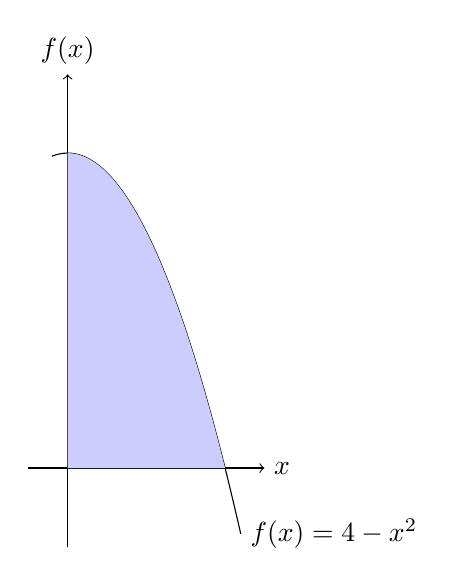
\begin{tikzpicture}
        \draw[->] (-0.5,0) -- (2.5,0) node[right] {$x$};
        \draw[->] (0,-1) -- (0,5) node[above] {$f(x)$};
        \draw[domain=-0.2:2.2, smooth, variable=\x, samples=100] plot ({\x}, {4 - \x*\x}) node[right] {$f(x) = 4 - x^2$};
        \fill[blue!20] (0,0) -- plot[domain=0:2, smooth] (\x, {4 - \x*\x}) -- (2,0) -- cycle;
    \end{tikzpicture}
    \end{center}
    
    \end{example}
\newpage


\subsubsection{Área entre dos curvas}

\begin{example}
    \textbf{Problema:} Calcular el área entre las curvas \( y = x \) y \( y = x^2 \) en el intervalo donde se intersectan.

\textbf{Solución:}
Primero, encontramos los puntos de intersección resolviendo \( x = x^2 \):

\[
x^2 - x = 0 \\
x(x - 1) = 0 \\
x = 0 \text{ o } x = 1
\]

El área entre las curvas se calcula como:

\[
\text{Área} = \int_{0}^{1} (x - x^2) \, dx
\]

Calculando la integral:

\[
\text{Área} = \left[ \frac{x^2}{2} - \frac{x^3}{3} \right]_{0}^{1} = \left(\frac{1}{2} - \frac{1}{3}\right) - (0 - 0) = \frac{1}{6}
\]

\begin{center}
\begin{tikzpicture}
    \begin{axis}[
        axis lines=middle,
        xlabel={$x$},
        ylabel={$y$},
        xmin=-0.1, xmax=1.2,
        ymin=-0.1, ymax=1.2,
        samples=100,
        domain=0:1,
        legend pos=outer north east
    ]
    \addplot[name path=f, domain=0:1, blue, thick] {x^2} node[pos=0.8, above right] {$y = x^2$};
    \addplot[name path=g, domain=0:1, red, thick] {x} node[pos=0.9, above right] {$y = x$};
    \addplot[blue!20] fill between[of=f and g, soft clip={domain=0:1}];
    \legend{$y = x^2$, $y = x$}
    \end{axis}
\end{tikzpicture}
\end{center}
\end{example}




\subsubsection{Volumen de sólidos de revolución.}
\begin{example}
    
    \textbf{Problema:} Calcular el volumen del sólido generado al girar la región bajo la curva \( y = x^2 \) desde \( x = 0 \) hasta \( x = 1 \) alrededor del eje \( x \).
    
    \textbf{Solución:}
    \[
    \text{Volumen} = \pi \int_0^1 (x^2)^2 \, dx = \pi \int_0^1 x^4 \, dx = \pi \left[ \frac{x^5}{5} \right]_0^1 = \frac{\pi}{5}
    \]
    
    \begin{center}
    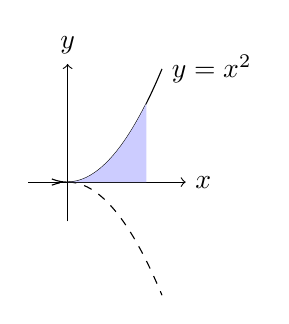
\begin{tikzpicture}
        \draw[->] (-0.5,0) -- (1.5,0) node[right] {$x$};
        \draw[->] (0,-0.5) -- (0,1.5) node[above] {$y$};
        \draw[domain=-0.2:1.2, smooth, variable=\x, samples=100] plot ({\x}, {\x*\x}) node[right] {$y = x^2$};
        \draw[domain=-0.2:1.2, smooth, variable=\x, samples=100, dashed] plot ({\x}, {-\x*\x});
        \fill[blue!20] (0,0) -- plot[domain=0:1, smooth] (\x, {\x*\x}) -- (1,0) -- cycle;
    \end{tikzpicture}
    \end{center}
    \end{example}
\newpage
\subsubsection{Longitud de una curva.}
\begin{example}    
    \textbf{Problema:} Calcular la longitud de la curva \( y = \ln(x) \) desde \( x = 1 \) hasta \( x = 2 \).
    
    \textbf{Solución:}
    \[
    \text{Longitud} = \int_1^2 \sqrt{1 + \left(\frac{d}{dx}(\ln(x))\right)^2} \, dx
    \]
    \[
    = \int_1^2 \sqrt{1 + \left(\frac{1}{x}\right)^2} \, dx = \int_1^2 \sqrt{1 + \frac{1}{x^2}} \, dx
    \]
    \[
    = \left[ \sqrt{x^2 + 1} \right]_1^2 = \sqrt{5} - \sqrt{2}
    \]
    
    \begin{center}
    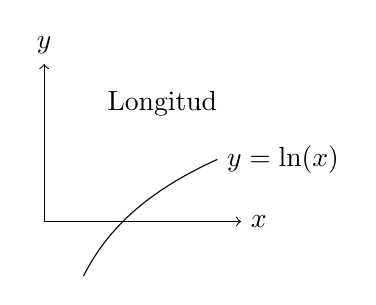
\begin{tikzpicture}
        \draw[->] (0,0) -- (2.5,0) node[right] {$x$};
        \draw[->] (0,0) -- (0,2) node[above] {$y$};
        \draw[domain=0.5:2.2, smooth, variable=\x, samples=100] plot ({\x}, {ln(\x)}) node[right] {$y = \ln(x)$};
        \node at (1.5,1.5) {Longitud};
    \end{tikzpicture}
    \end{center}
    \end{example}


\subsubsection{Integral impropia}

\begin{definition}[Integral impropia]
    Es una integral definida en la cual uno o ambos de los límites de integración son infinitos, o la función integrando tiene una discontinuidad en el intervalo de integración.
\end{definition}
Formalmente, se definen dos tipos principales de integrales impropias:

\subsubsection{Integrales con límites infinitos:}
\begin{align}
    &\int_{a}^{\infty} f(x) \, dx \\
    &\int_{-\infty}^{b} f(x) \, dx
\end{align}
Estas integrales se definen como el límite de integrales definidas cuando el límite superior o inferior tiende a infinito:
\begin{align}
    &\int_{a}^{\infty} f(x) \, dx = \lim_{b \to \infty} \int_{a}^{b} f(x) \, dx\\
    &\int_{-\infty}^{b} f(x) \, dx = \lim_{a \to -\infty} \int_{a}^{b} f(x) \, dx
\end{align}

\subsubsection{Integrales con discontinuidades en el intervalo de integración:}
   Si la función tiene discontinuidades en el intervalo \([a, b]\), se dividen las integrales en intervalos donde la función es continua, y se toman los límites en los puntos de discontinuidad:
 \begin{equation}
    \int_{a}^{b} f(x) \, dx = \lim_{\epsilon \to 0^+} \left(\int_{a}^{c - \epsilon} f(x) \, dx + \int_{c + \epsilon}^{b} f(x) \, dx\right)
 \end{equation}
   donde \(c\) es el punto de discontinuidad.

\subsubsection{Integral con Límite Superior Infinitamente Grande}

\begin{example}
    \textbf{Problema:} Calcular la integral impropia
\[
\int_{1}^{\infty} \frac{1}{x^2} \, dx
\]

\textbf{Solución:}
\[
\int_{1}^{\infty} \frac{1}{x^2} \, dx = \lim_{b \to \infty} \int_{1}^{b} \frac{1}{x^2} \, dx
\]
Calculando la integral definida:
\[
\int_{1}^{b} \frac{1}{x^2} \, dx = \left[ -\frac{1}{x} \right]_{1}^{b} = -\frac{1}{b} + 1
\]
Tomando el límite cuando \( b \to \infty \):
\[
\lim_{b \to \infty} \left(-\frac{1}{b} + 1\right) = 1
\]
Entonces,
\[
\int_{1}^{\infty} \frac{1}{x^2} \, dx = 1
\]

\begin{center}
\begin{tikzpicture}
    \begin{axis}[
        axis lines=middle,
        xlabel={$x$},
        ylabel={$y$},
        xmin=0, xmax=3,
        ymin=0, ymax=2,
        samples=100,
        domain=0.1:3,
        legend pos=outer north east
    ]
    \addplot[name path=f, domain=0.1:3, blue, thick] {1/x^2} node[pos=0.9, above right] {$f(x) = \frac{1}{x^2}$};
    \addplot[name path=g, domain=1:3, opacity=0] {0};
    \addplot[blue!20] fill between[of=f and g, soft clip={domain=1:3}];
    \legend{$f(x) = \frac{1}{x^2}$}
    \end{axis}
\end{tikzpicture}
\end{center}
\end{example}

\subsubsection{Integral con Discontinuidad}

\begin{example}
    \textbf{Problema:} Calcular la integral impropia
\[
\int_{0}^{1} \frac{1}{\sqrt{x}} \, dx
\]

\textbf{Solución:}
\[
\int_{0}^{1} \frac{1}{\sqrt{x}} \, dx = \lim_{\epsilon \to 0^+} \int_{\epsilon}^{1} \frac{1}{\sqrt{x}} \, dx
\]
Calculando la integral definida:
\[
\int_{\epsilon}^{1} \frac{1}{\sqrt{x}} \, dx = \left[ 2\sqrt{x} \right]_{\epsilon}^{1} = 2 - 2\sqrt{\epsilon}
\]
Tomando el límite cuando \( \epsilon \to 0^+ \):
\[
\lim_{\epsilon \to 0^+} (2 - 2\sqrt{\epsilon}) = 2
\]
Entonces,
\[
\int_{0}^{1} \frac{1}{\sqrt{x}} \, dx = 2
\]

\begin{center}
\begin{tikzpicture}
    \begin{axis}[
        axis lines=middle,
        xlabel={$x$},
        ylabel={$y$},
        xmin=-0.1, xmax=1.1,
        ymin=0, ymax=4,
        samples=100,
        domain=0.01:1,
        legend pos=outer north east
    ]
    \addplot[name path=f, domain=0.01:1, red, thick] {1/sqrt(x)} node[pos=0.9, above right] {$f(x) = \frac{1}{\sqrt{x}}$};
    \addplot[name path=g, domain=0.01:1, opacity=0] {0};
    \addplot[red!20] fill between[of=f and g, soft clip={domain=0.01:1}];
    \legend{$f(x) = \frac{1}{\sqrt{x}}$}
    \end{axis}
\end{tikzpicture}
\end{center}
\end{example}













